\begin{figure}[!htbp]
\centering
\begin{subfigure}[b]{\linewidth}
  \centering
  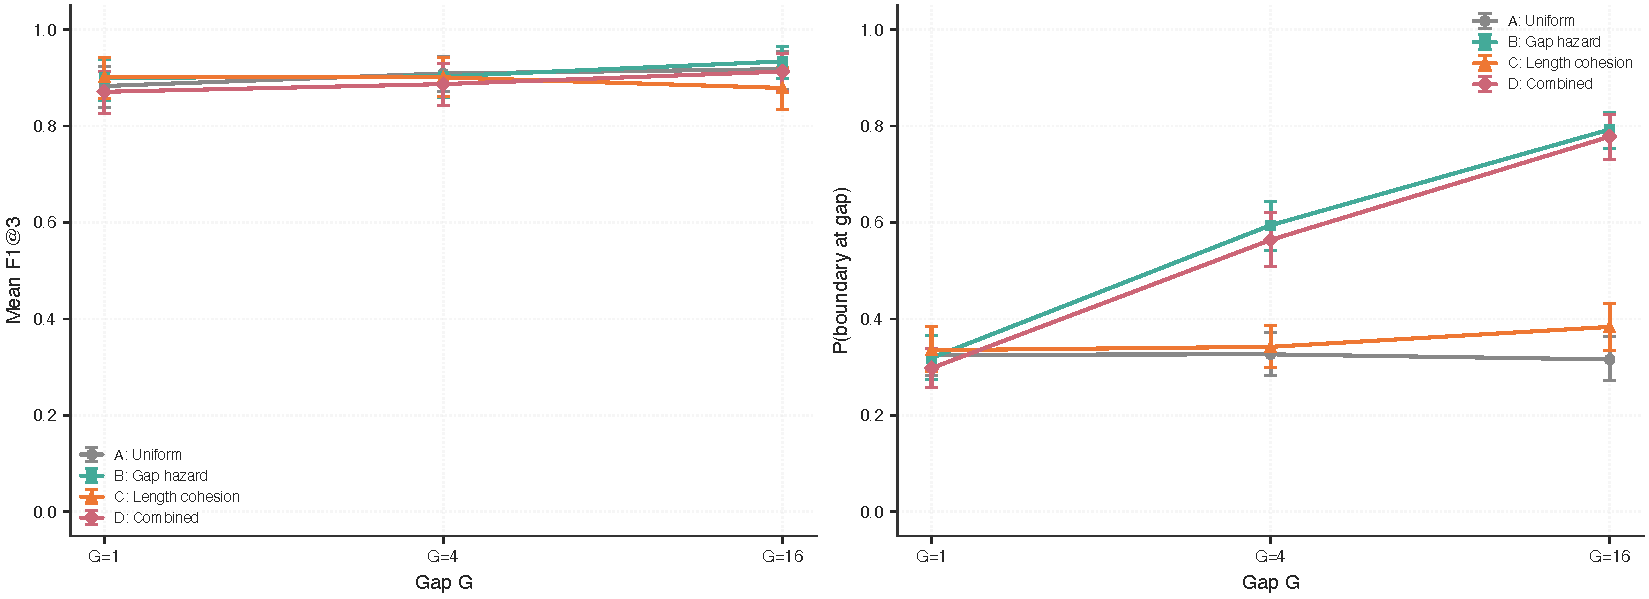
\includegraphics[width=\linewidth]{figures/fig_E03_gap_true.pdf}
  \caption{True changepoint at the gap location ($i=120$). Posterior boundary probability
  increases with gap size $G$ under gap-hazard (B) and combined (D) priors.}
  \label{fig:E03-gap-true-paper}
\end{subfigure}
\vspace{4pt}
\begin{subfigure}[b]{\linewidth}
  \centering
  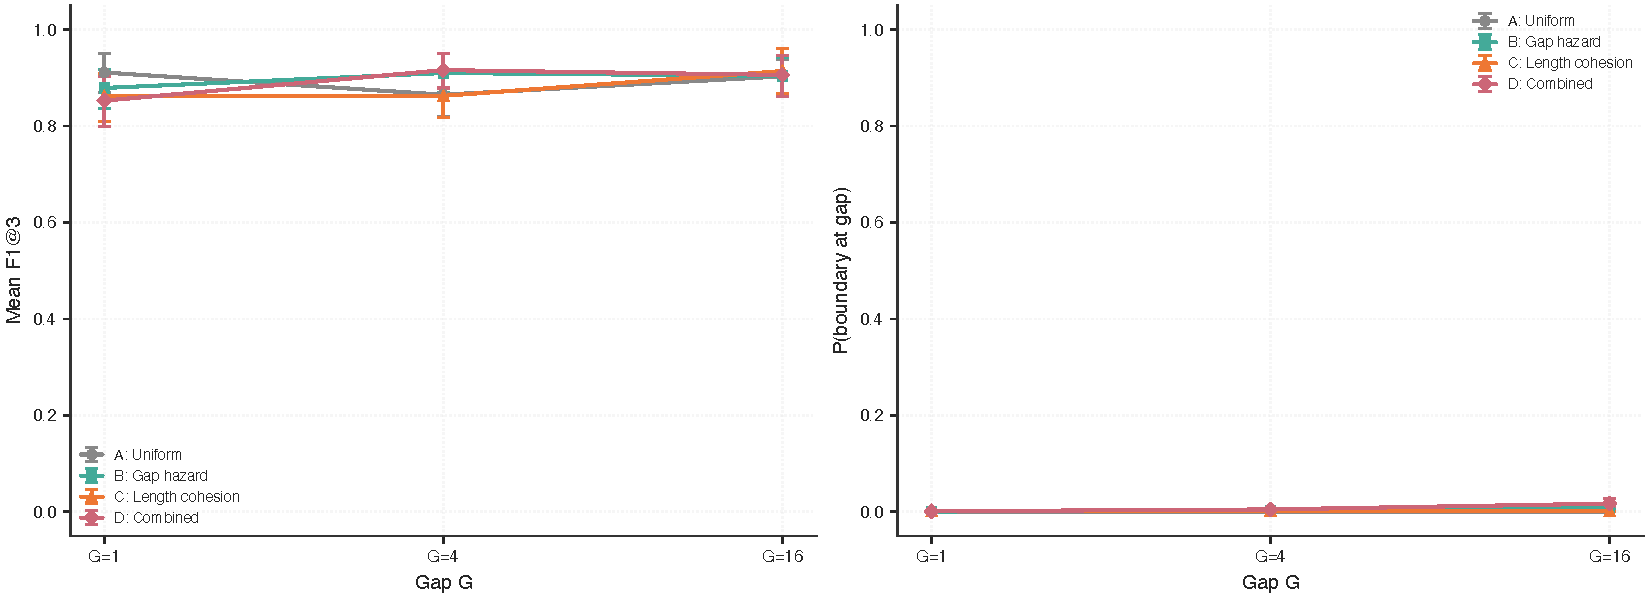
\includegraphics[width=\linewidth]{figures/fig_E03_gap_false.pdf}
  \caption{No changepoint at the gap location. All four priors assign near-zero
  posterior probability at $i=120$ regardless of gap size.}
  \label{fig:E03-gap-false-paper}
\end{subfigure}
\caption{Irregular-design prior ablation. Mean boundary posterior $P(b_{120}=1\mid y)$
with 95\% bootstrap bands across 100 independent datasets. Top panel: generating template
places a true changepoint at the large-gap position (boundaries 60,\,120); gap-hazard
and combined priors correctly raise posterior probability at the gap when evidence
supports a change. Bottom panel: generating template places no changepoint at the gap
(boundaries 60,\,180); all priors correctly preserve near-zero false-positive probability.
Mean $\mathrm{F_1}@3$ exceeds $0.85$ in every cell under all four priors.}
\label{fig:E03-irregular-paper}
\end{figure}
